\documentclass[a4paper,12pt]{article}
\title{\textbf{Bioimpresi\'{o}n 3d aplicada al campo Card\'{i}aco}\\\large{ECB, EMDTB, SHB || Q6 EEBE - UPC}}
\author{Oriol Ruiz Dom\'{i}nguez}

\usepackage[section]{placeins}
\usepackage{mathtools}
\usepackage{hyperref}
\usepackage[utf8]{inputenc}
\usepackage{lmodern}
\usepackage[spanish]{babel}
\usepackage[left=1.5cm,top=2.5cm,right=1.5cm,bottom=2.5cm]{geometry} 
\usepackage{amsmath,amssymb,amsthm,textcomp}
\usepackage{graphicx}
\usepackage{eurosym}
\usepackage{listings} 
\providecommand{\abs}[1]{\lvert#1\rvert}
\usepackage{color} %red, green, blue, yellow, cyan, magenta, black, white
\definecolor{mygreen}{RGB}{28,172,0} % color values Red, Green, Blue
\definecolor{mylilas}{RGB}{170,55,241}

%Extra levels of subsection
\usepackage{titlesec}
\setcounter{secnumdepth}{4}
\titleformat{\paragraph}
{\normalfont\normalsize\bfseries}{\theparagraph}{1em}{}
\titlespacing*{\paragraph}
{0pt}{3.25ex plus 1ex minus .2ex}{1.5ex plus .2ex}

\begin{document}
\maketitle
\pagebreak
\tableofcontents
\pagebreak
\listoffigures
\pagebreak


\pagebreak
\section{Introducción}

\pagebreak
\section{Historia}

\subsection{Historia de los biomateriales}

\subsection{Historia de la impresión y bioimpresión 3D}

\subsection{Biomateriales e impresión 3D en el campo vascular}

\pagebreak
\section{Marco actual - Investigación y mercado}

\pagebreak
\section{Marco legal - Nivel de mercado. Normativa}

\pagebreak
\section{Fisiología}

\subsection{El sistema circulatorio}

\subsection{El corazón}

\subsubsection{Función del corazón}

\subsubsection{Anatomía del corazón}

\subsubsection{Actividad eléctrica del corazón (Potenciales de acción cardíacos)}

\subsubsection{Mecanismo de contracción cardíaco}

\subsubsection{Ciclo cardíaco}

\subsection{Problemas y enfermedades cardíacas}

\pagebreak
\section{Biomateriales y Biocompatibilidad}

\subsection{Principales materiales para bioimpresión}

\subsubsection{Cerámicos}

\subsubsection{Polímeros}

\subsubsection{Metales}

\subsubsection{Hidrogeles}

\subsection{Biocompatibilidad}

\subsection{Ventajas e inconvenientes de los biomateriales}

\subsection{Impresión de stents}

\subsubsection{Metodología}

\subsubsection{Materiales empleados}

\subsubsection{Ventajas e inconvenientes de Stents 3D}

\pagebreak
\section{Bioimpresión}
\subsection{Estrategias de bioimpresión}
La bioimpresión se basa en la deposición de material biológico siguiendo un patrón establecido. Existen variedad de métodos que cumplen este objetivo, aunque los principales son: por inyección de tinta, mediante microextrusión o bien mediante un láser.

	\begin{figure}[!ht]
	\begin{center}
	  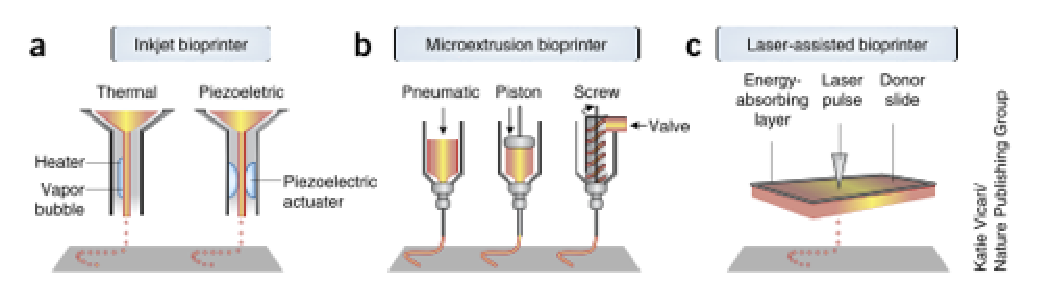
\includegraphics[width=0.5\textwidth]{Figuras/tiposBioimpresion.eps}
	  \caption{\emph{Estrategias de bioimpresión. }Extraído de \emph{---FALTA CITAR---}.}
	\end{center}
	\label{tiposBioimpresion}
	\end{figure}

\subsubsection{Inyección de tinta}
Las impresoras de inyección de tinta son el modelo más empleado en el ámbito no biológico. De hecho, las primeras bioimpresoras de inyección de tinta se crearon a partir de la modificación de impresoras comerciales. Su funcionamiento consiste en la deposición de un volumen de tinta controlado en la posición establecida.

Para realizar la eyección de tinta hay dos métodos: térmica y acústicamente.

\paragraph{Inyección térmica}
El método térmico consiste en calentar eléctricamente el cabezal entre 200 y 300 grados para realizar pulsos de presión y que caiga el material. Estudios han demostrado que esta temperatura, al producirse en alrededor de 2$\mu s$ y estar tan localizada, no tiene gran impacto en la estabilidad de las moléculas biológicas, como el ADN ya que solo provocan un incremento de entre 4 y 10 ºC.


\paragraph{Inyección acústica}
Otra manera de realizar inyección de volumen de líquido controlado es mediante un cristal piezoeléctrico. Al aplicarle un voltaje a este piezoeléctrico este produce una onda acústica, así como un cambio rápido en su forma de manera que genera la presión suficiente como para eyectar el líquido. También es posible realizar la presión mediante una fuerza de radiación acústica asociada a los ultrasonidos.

Varios parámetros como el pulso, la duración o la amplitud se ajustan para controlar el volumen de eyección y la frecuencia a la que se producen.

\subsubsection{Microextrusión}

\subsubsection{Láser}

\subsection{Impresoras}
El mercado actual de impresión 3d está creciendo exponencialmente dado al reducido precio al que se ha conseguido diseñar los equipos. Hay diferentes empresas destinadas al sector, aunque hay que hacer una mención especial a las impresoras diseñadas en la plataforma open-source reprap.org, en la cuál se puede encontrar un ámplio abanico de diseños de manera gratuita.

Uno de los modelos más fabricados es la impresora Prusa I3 bajo la licencia de reprap, diseñada por el CEO de PrusaResearch Josef Průša. Dada la facilidad de acceso a las diferentes partes del equipo y la posibilidad de cambiar sus partes, estos modelos han sido empleados por muchas empresas tanto para ser comercializados como para la creación de impresoras adaptadas para realizar bioimpresión.

Más allá de las impresoras open-source, empresas como BCN3D (bajo la FundacióCIM-UPC), han desarrolado impresoras como la BCN3D Sigma. De nuevo, los modelos básicos no suelen estar diseñados para realizar bioimpresión, pero en laboratorios como el del Dr Gioseppe Scionti realizan la adaptación para ello.

\subsubsection{Partes básicas}
Todos los modelos más comerciales de impresoras 3d cuentan con unas especificaciones similares. Es necesario es necesario tener un cabezal de impresión (habitualmente extrusor), una superficie de soporte (habitualmente cama caliente), servomotores (habitualmente 5), una placa controladora y la estructura.

Para poder realizar una impresión 3d es necesario tener movimiento en 3 ejes (x, y, z). Los diferentes modelos de impresión suelen diferir en qué se mueve de la impresora (el cabezal, el soporte…), pero el modelo generalizado realiza movimiento del cabezal en los ejes x (un servomotor) y z (dos servomotores), mientras que para el eje y se mueve el soporte (un servomotor). El servomotor restante es el que controla la cantidad de material a poner en el modelo.

	\begin{figure}[!ht]
	\begin{center}
	  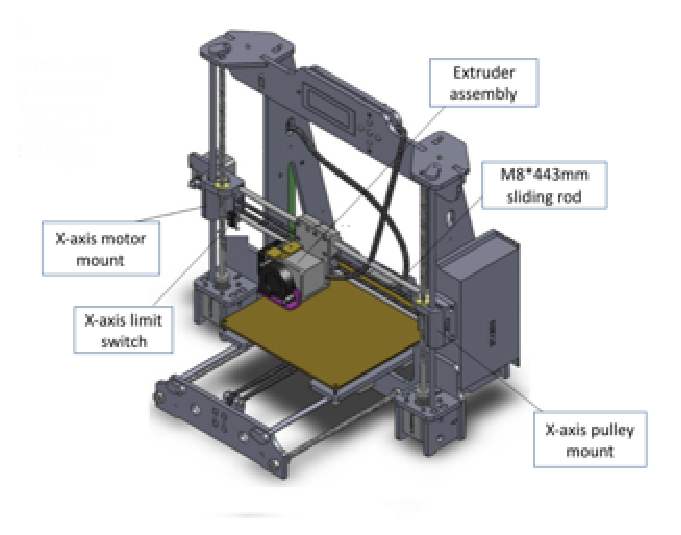
\includegraphics[width=0.5\textwidth]{Figuras/partesImpresora.eps}
	  \caption{\emph{Partes de una impresora. }Extraído de \emph{Manual de montaje Tronxy P802MA}.}
	\end{center}
	\label{partesImpresora}
	\end{figure}


\subsubsection{Placas}
Para poder realizar el control de la impresora se deben conectar todos sus elementos a un controlador. Existen variedad de modelos diferentes en función de las prestaciones que busquemos (visitar http://reprap.org/wiki/Comparison_of_Electronics para ver las diferencias entre ellas), aunque despunta el uso de una placa en concreto: RAMPS.\\

RAMPS es el acrónimo de \emph{RepRap Arduino Mega Pololu Shield}, es decir, es una placa desarrollada por RepRap basada en Arduino Mega con el módulo Pololu. Al estar basada en una placa como Arduino Mega, su coste es muy reducido aunque a su vez tiene un elevado potencial de expansión. Asimismo, su diseño es totalmente modular, por lo que es la manera más sencilla de cambiar los elementos de la impresora, como pueden ser los drivers de los motores paso a paso. A Mayo 2017 sigue en fase de desarrollo, estando lanzada oficialmente la versión 1.4. Pueden encontrarse modificaciones de esta, como la versión 1.4.2 (Figura \ref{figure:Ramps142}) u otras versiones modificadas que se venden en tiendas online, principalmente de origen chino.\\

	\begin{figure}[!ht]
	\begin{center}
	  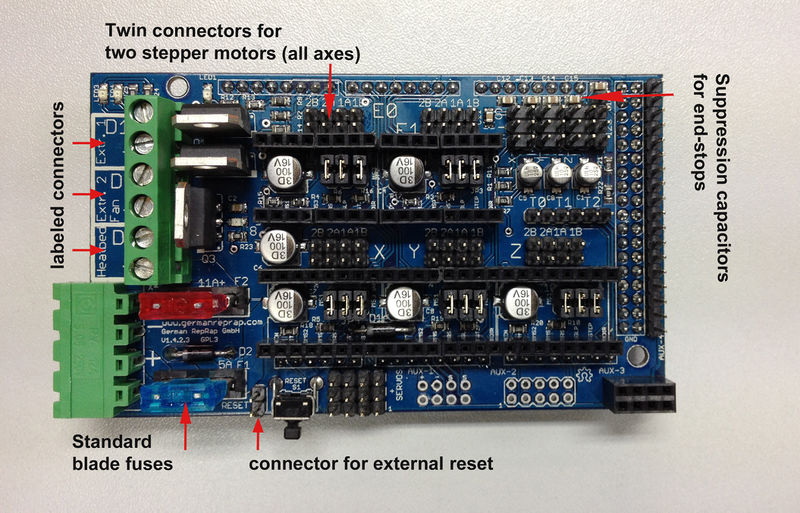
\includegraphics[width=0.75\textwidth]{Figuras/RAMPS_142.jpg}
	  \caption{\emph{Ramps 1.4.2}}
	\end{center}
	\label{figure:Ramps142}
	\end{figure}

\begin{itemize}
	\item \textbf{Controlador}

	El controlador de Arduino Mega es un ATmega2650. Este controlador cuenta con las especificaciones citadas en el cuadro \ref{table:ATmega2650} (datos obtenidos en la  \emph{\href{https://www.arduino.cc/en/Main/arduinoBoardMega2560}{página web de Arduino}}).

\begin{table}[h!]
\begin{center}
\begin{tabular}{ |l|c|l| }
\hline
Microcontroller & ATmega2650 & Observations \\ 
\hline
Operating Voltage & 5V & \\
Input Voltage (recommended) & 7-12V & \\
Input Voltage (limit) & 6-20V & \\
Digital I/O Pins & 54 & 15 provide PWM output\\
Analog Input Pins & 16 & \\
DC Current per I/O Pin & 20 mA & \\
DC Current for 3.3V Pin & 50 mA & \\
Flash Memory & 256 KB & 8 KB used by bootloader\\
SRAM & 8 KB & \\
EEPROM & 4 KB & \\
Clock Speed & 16 MHz & \\
LED BUILTIN & 13 & \\
Length & 101.52 mm & \\
Width & 53.3 mm & \\
Weight & 37 g & \\
\hline
\end{tabular}
\caption{Especificaciones del microcontrolador ATmega2650}
\label{table:ATmega2650}
\end{center}
\end{table}


\item \textbf{Circuitería}

En la propia página de RAMPS podemos encontrar diagramas esquemáticos del diseño de la placa.\\

En el diagrama de Conectores (Figura \ref{RAMPS_connectors}) podemos apreciar la agrupación de pins por los diferentes módulos con los que va a tratar.

Por otro lado, en la Figura \ref{RAMPS_bothsides} se sobrepone el circuito impreso que ocupa la parte inferior de la placa, realizando así las conexiones necesarias entre los pins.

Finalmente, en la Figura \ref{RAMPS_schematic} encontramos los diferentes módulos por bloques.

\end{itemize}


	\begin{figure}[!ht]
	\begin{center}
	  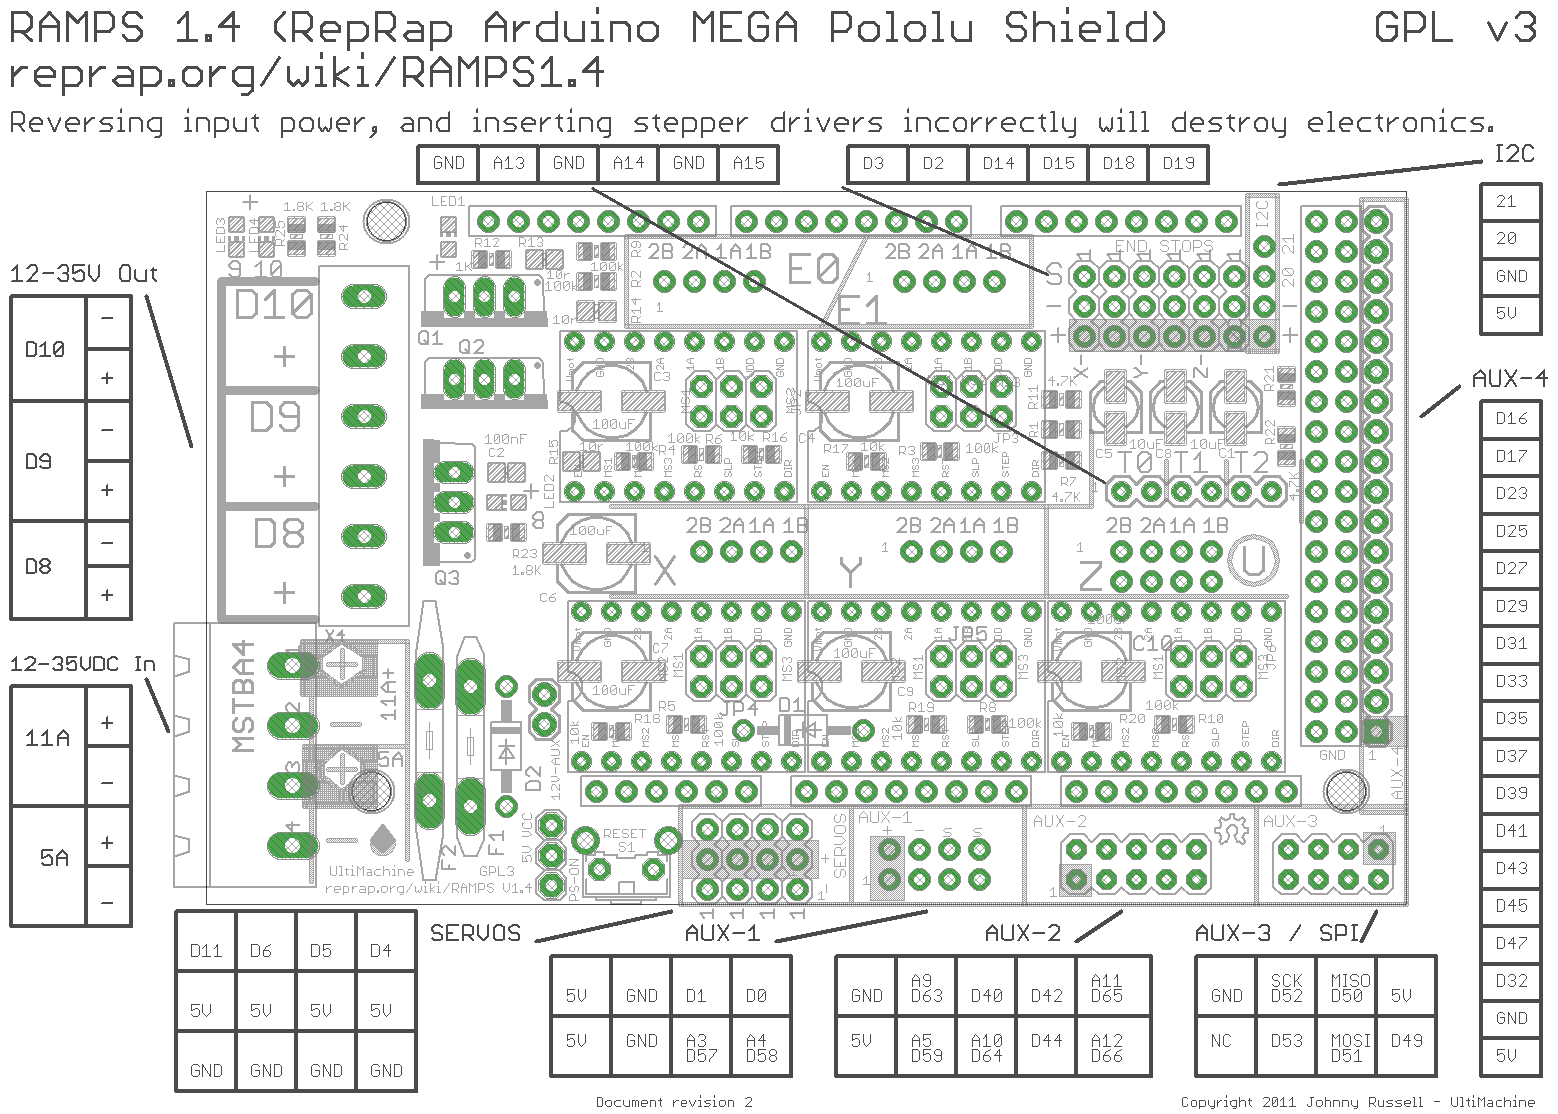
\includegraphics[width=0.8\textwidth]{Figuras/RAMPS_14_connectors.png}
	  \caption{\emph{RAMPS 1.4: Conectores}}
	\end{center}
	\label{RAMPS_connectors}
	\end{figure}
	
	
	\begin{figure}[!ht]
	\begin{center}
	  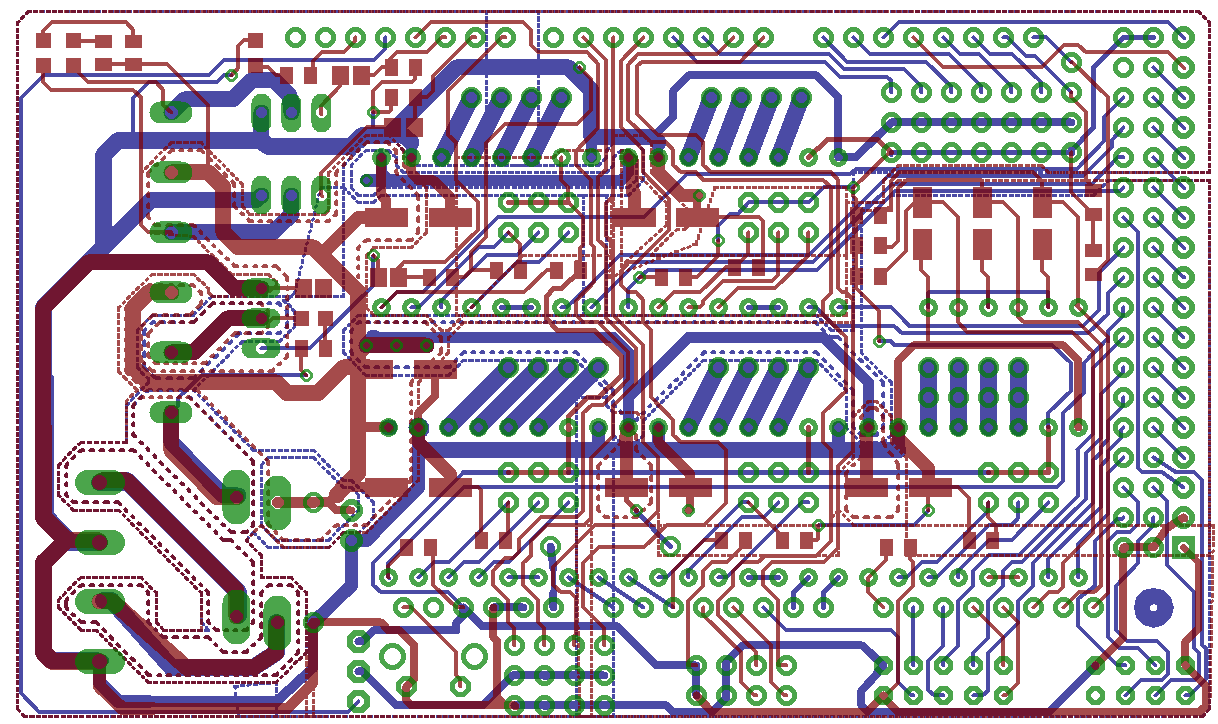
\includegraphics[width=0.8\textwidth]{Figuras/RAMPS_14_bothsides.png}
	  \caption{\emph{RAMPS 1.4: Circuito impreso}}
	\end{center}
	\label{RAMPS_bothsides}
	\end{figure}
	
	
	\begin{figure}[!ht]
	\begin{center}
	  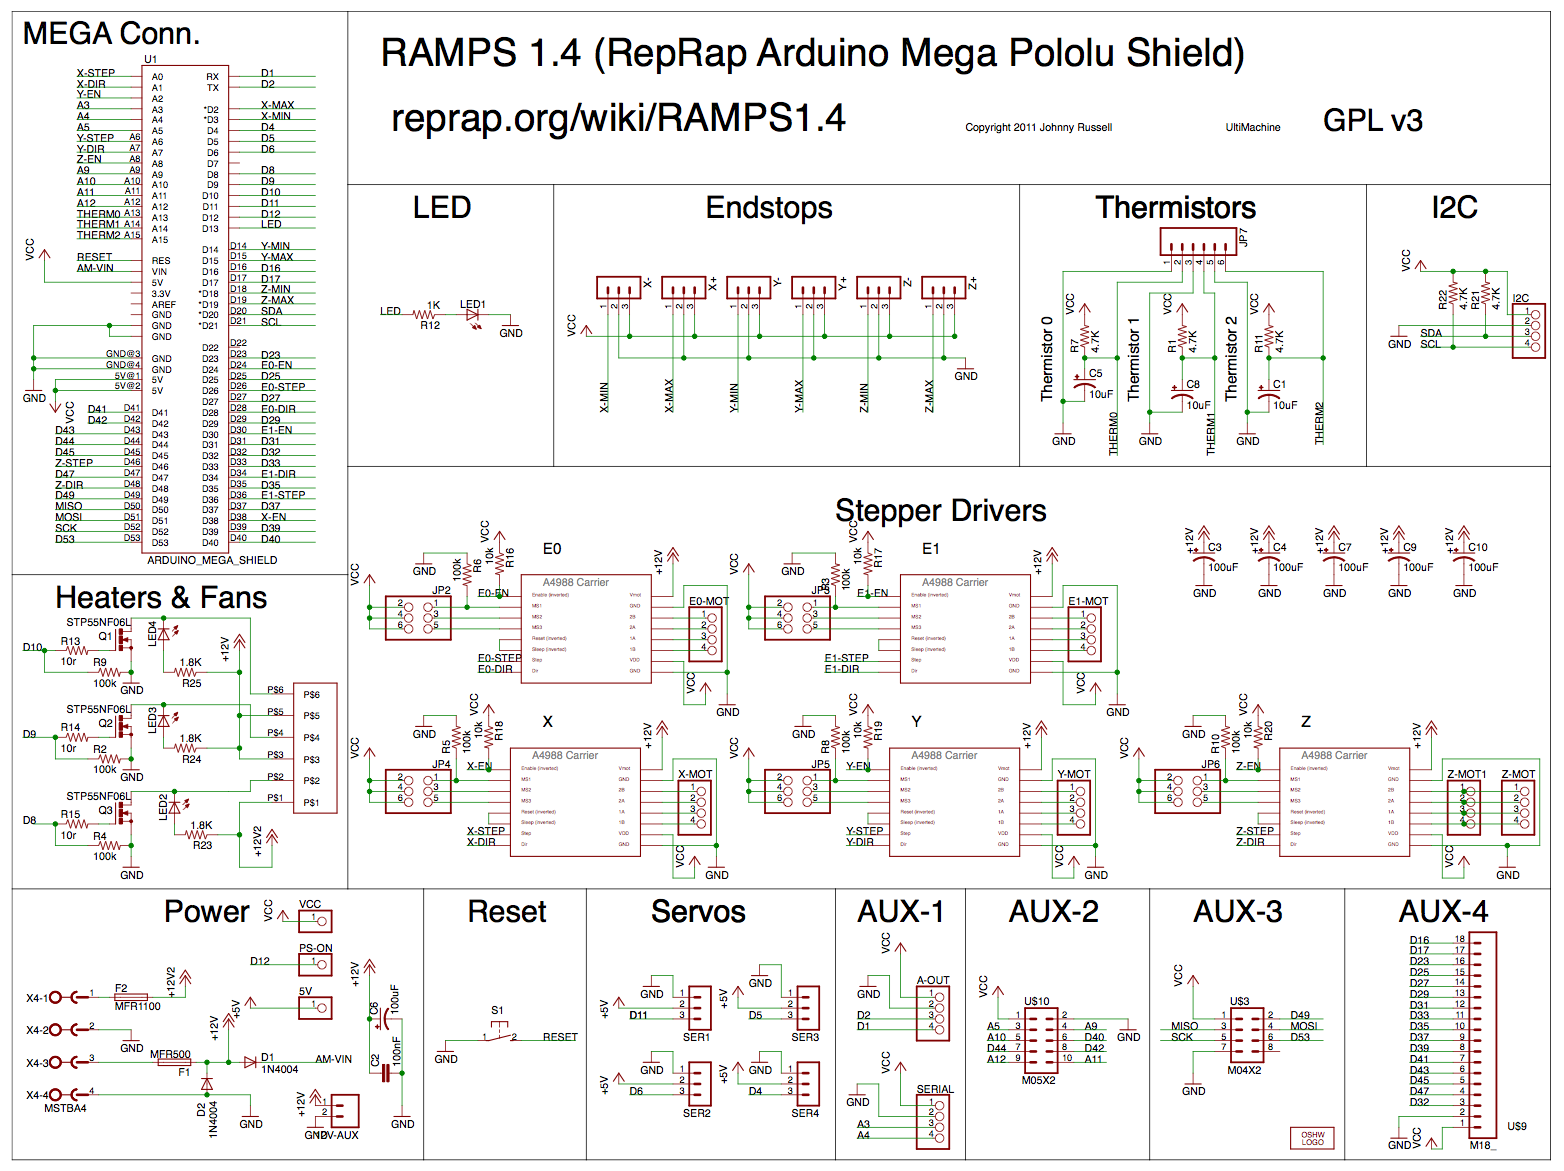
\includegraphics[width=0.9\textwidth]{Figuras/RAMPS_14_schematic.png}
	  \caption{\emph{RAMPS 1.4: módulos por bloques}}
	\end{center}
	\label{RAMPS_schematic}
	\end{figure}

Otras placas ofrecen prestaciones como conectividad WiFi \emph{(DuetWifi)} o el hecho de tenerlo todo en una misma placa \emph{(Melzi)}.\\


\subsubsection{Firmware}
Una vez se tienen el hardware necesario para montar la impresora, es necesario ponerle firmware para que comprenda qué movimientos debe realizar.\\

De nuevo, existen una amplia variedad de opciones a instalar, pero hay proyectos que despuntan en cantidad de usuarios y que el crecimiento de su comunidad avanza exponencialmente. Ejemplos de ello son \emph{Marlin} y \emph{Repetier}.\\

\paragraph{Marlin}
Marlin es un firmware mantenido por la comunidad RepRap para impresoras 3D basadas en Arduino, dando soporte a los microcontroladores de RAMPS, RAMBo, Ultimaker o BQ entre otras. Interpreta los archivos a imprimir mediante USB o tarjetas MicroSD. Está basado en el proyecto \emph{Sprinter}, y tiene licencia GNU GPL v3.\\

Marlin es un proyecto todavía en desarrollo. La última release publicada a Mayo 2017 es la 1.0.2.

Para obtener la última versión, así como las que se han publicado anteriormente, se recomienda acceder a su repositorio hospedado en GitHub (\href{https://github.com/MarlinFirmware/Marlin/}{https://github.com/MarlinFirmware/Marlin/}).\\

Al tener todo el código abierto, muchas compañías ofrecen sus impresoras con modificaciones en el firmware. Habitualmente pueden ser encontradas en clones de este proyecto, o bien a través de ramas de estos. No obstante, estos cambios no suelen ir más allá que cambiar el sentido del movimiento de un servo-motor, o bien de activar (o desactivar) un sensor de proximidad inductivo en un eje (como puede ser el z) como cambio a un final de carrera.\\


\paragraph{Repetier}
Repetier.com es un proyecto mantenido por la empresa alemana \emph{Hot-World GmbH and Co}. Esta empresa ofrece una suite completa para controlar la impresora, abarcando diferentes módulos entre los cuales se encuentran \emph{Repetier-Host}, \emph{Repetier-Firmware} o \emph{Repetier-Server}. Los módulos pueden ser instalados independientemente, aunque cuando se opta por contar con esta tecnología es habitual instalarlos todos.\\

\emph{Repetier-Firmware} se corresponde con la parte que se debe instalar en el controlador (como por ejemplo, RAMPS) para procesar los datos e imprimir. 

Por otro lado, \emph{Repetier-Server} es un instalador para crear un servidor mediante el cual, al estar conectado a la impresora y a la red, se pueda acceder a la impresora y controlar sus movimientos desde otros dispositivos.

Finalmente, \emph{Repetier-Host} ofrece la interfaz de escritorio para diferentes sistemas operativos (Windows, Linux y OSX) para poder enviar los datos a la impresora, pasando anteriormente por \emph{Repetier-Server} si se pretende hacer de manera inhalámbrica.


\subsubsection{Adaptación a la bioimpresión de stents}
Para poder realizar una bioimpresión de stents con una impresora 3d será necesario realizar modificaciones en la impresora que se disponga, pues con las que hay comercialmente no se pueden conseguir los resultados necesarios. Dado a que se debe modificar el sistema, es habitual encontrar laboratorios que modifican equipos del proyecto RepRap, dado que al ser de código libre es mucho más fácil acceder a sus esquemas para poder estudiar qué modificaciones deberán realizarse.\\

Asimsimo, al trabajar con impresoras del proyecto RepRap se puede contar con el firmware Marlin, que como se ha citado es mantenido por la misma organización, y también contará con el código abierto para poder realizar los cambios que sean necesarios. En el laboratorio del Dr Scionti, por ejemplo, hemos podido observar uno de estos cambios para adaptar una impresora 3d convencional a una de bioimpresión de stents.\\

\paragraph{Cambios mecánicos}
Las impresoras 3d por excelencia, las más comercializadas, son las de bobina de hilo. No obstante, para ser capaces de imprimir stents con PLLA deberemos cambiar el sistema de alimentación. Dada la volatilidad de este material, será preferible trabajar con él mediante una impresión por microextrusión con pistón mecánico.\\

El primer paso consiste en modificar el servo-motor de extrusión mediante un sistema de engranajes, de manera que estos acaben moviendo ligeramente un pistón.

%%%% INSERTAR FIGURA %%%%

Por otro lado, el eje $y$ que habitualmente es movido por una cama se debe retirar. En su lugar se pne una barra cilíndrica que abarca todo el ancho de la impresora. Esta será movida por otro servo-motor, y es preferible que en los extremos cuente con cojinetes de manera que su giro sea lo más regular posible.

	\begin{figure}[!ht]
	\begin{center}
	  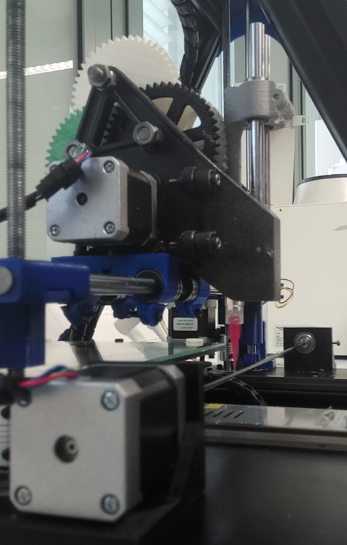
\includegraphics[width=0.5\textwidth]{Figuras/stents_adapt.png}
	  \caption{\emph{Bioimpresora adaptada para stents}}
	\end{center}
	\label{stents_adapt}
	\end{figure}


\paragraph{Cambios de firmware}
Al haber realizado cambios en los servo-motores del sistema, deberemos volver a calibrar la impresora. Los servo-motores, y en especial los de precisión, cuentan con una cantidad de posiciones o cuentas de posibles posiciones para cada mm. Conociendo este ajuste de cuentas, en el firmware de la impresora debemos ajustar cuántas se deben avanzar para poder mover una cantidad exacta de distancia en la realidad.\\

Ya sea mirando las especificaciones de los servo-motores empleados o bien mediante una calibración prueba-error, debemos llegar a conocer las cuentas por milímetro de nuestros motores. Llegados a este punto, deberemos introducir el valor en el firmware para que cuando esta mande la orden de avanzar un milímetro realice realmente este movimiento.\\

Para ello, deberemos acceder al código de Marlin. Estando en su repositorio, y habiendo descargado la rama que queremos montar en nuestra impresora, deberemos acceder a la carpeta "/Marlin". Dentro de esta se encuentra un archivo llamado \emph{"Configuration.h"}, el cual deberemos modificar con un editor de texto.\\

En este archivo encontraremos una línea de código en la cuál se espeficican las cuentas. Esta es, por defecto:
\begin{lstlisting}
#define DEFAULT_AXIS_STEPS_PER_UNIT   { 80, 80, 4000, 500 }
\end{lstlisting}

Los valores definidos se corresponden respectivamente con las cuentas por unidad de los ejes $x$, $y$, $z$ y del extrusor. Para obtener el valor de estas deberemos realizar una serie de cálculos, tales como:

$$ \text{\textbf{Pasos por unidad (ejes X e Y)}} = \frac{\text{Pasos por unidad  (ejes X e Y)}}{\text{(Dientes de la polea)}\cdot \text{(Paso de la correa)}}$$
	
$$ \text{\textbf{Pasos por unidad (eje Z)}} = \frac{\text{Pasos del motor por revolución}}{\text{Paso de la varilla}}$$
	
$$ \text{\textbf{Pasos por unidad (extrusora)}} = \frac{\text{Pasos del motor por revolución} \cdot \text{ Relación de engranaje}}{\text{Diámetro de la rueda de apriete}\cdot \pi}$$



\FloatBarrier
\subsection{Modelado}
Otro pilar fundamental cuando se habla de impresión 3D son los modelos que se emplean. Estos pueden ser muy diferentes, siendo así su método de obtención totalmente distinto en función de qué estemos buscando. Habitualmente se crean modelos directamente desde un ordenador, con programas como \emph{Solidworks} o \emph{Autodesk Fusion} para modelos mecánicos o bien \emph{Blender} o \emph{3Ds Max} para figuras más gráficas.\\

Por otro lado, en el ámbito de la bioimpresión trataremos más habitualmente con diseños que en vez de crearse desde cero parten de una base: el paciente. Pueden obtenerse imágenes médicas mediante TACs, Resonancias Magnéticas o Angiografías, y a partir de estas crear el modelo del individuo de estudio. Por esta razón, diferenciamos entre el proceso para obtener un modelo de corazón o bien de stent cardíaco.\\

\subsubsection{Modelado cardíaco}
\emph{Nota: el proceso aquí descrito no es necesariamente el mejor ni el más rápido, sino el que se ha considerado mejor y más optimizado. Existen programas que crean el modelo .stl directamente desde imágenes DICOM, pero han sido rechazados en este trabajo debido a la falta de rigurosidad a la hora de analizar la validez de los datos.}\\

Habiendo realizado la adquisición de datos de nuestro paciente, es muy habitual recibir imágenes en formato DICOM. Para visualizar estas imágenes es necesario contar con un software que visualice los archivos y sea capaz de crear una reconstrucción a partir de las capturas de las diversas capas. Para dicha tarea destaca el software \href{http://www.osirix-viewer.com/}{OsiriX}, mediante el cual podremos obtener la imagen 3D en un formato \empn{.wrl}.\\

A partir de aquí comienza el proceso más complicado del modelaje cardíaco 3D. Las imágenes obtenidas cuentan con diversidad de impurezas, las cuales pueden ser desde errores en la obtención o el procesado hasta tejido duro indeseado. Es por ello que se realiza una fase de limpieza y suavizado del modelo. Un programa que nos permite hacer esta tarea es \href{https://www.blender.org/}{Blender}, el cual es un programa Open Source en 3D ya que permite crear modelos, animaciones, renderizar, crear vídeos o incluso juegos. Además, nos permite abrir nativamente el formato de archivo .wrl sin necesidad de realizar ningún tipo de conversión.\\

	\begin{figure}[!ht]
	\begin{center}
	  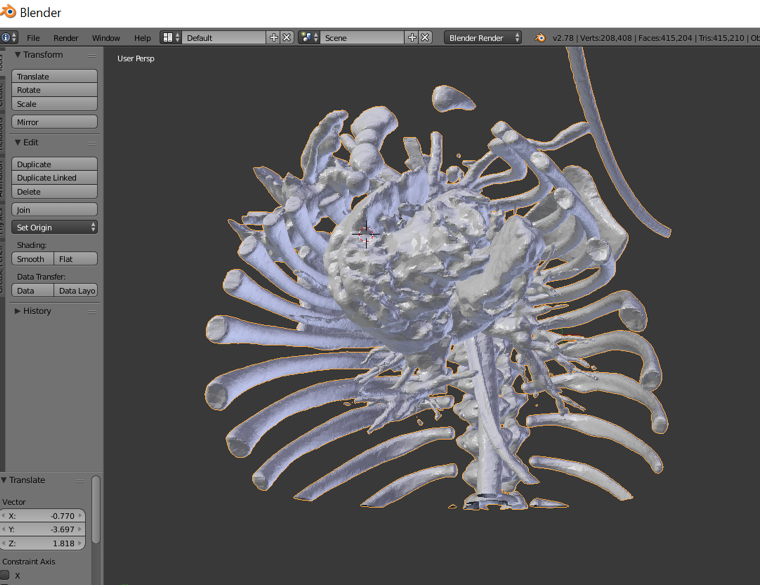
\includegraphics[width=0.75\textwidth]{Figuras/mod_01.png}
	  \caption{\emph{Modelo 3d sin tratar}}
	\end{center}
	\label{fig:mod_01}
	\end{figure}

	\begin{figure}[!ht]
	\begin{center}
	  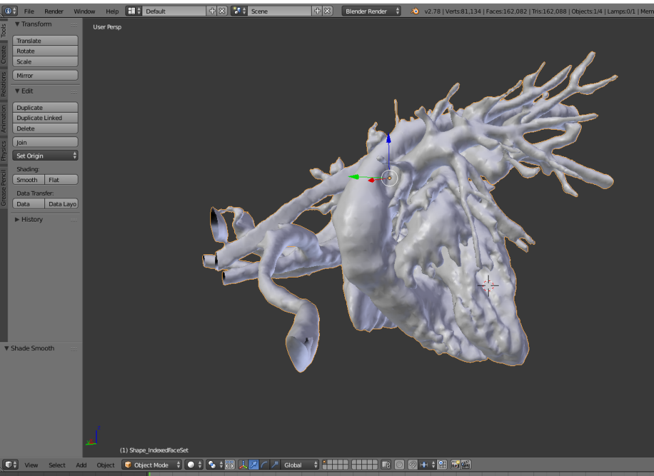
\includegraphics[width=0.75\textwidth]{Figuras/mod_02.png}
	  \caption{\emph{Modelo 3d tras eliminar las partes no deseadas}}
	\end{center}
	\label{fig:mod_02}
	\end{figure}


Teniendo abierto el archivo de corazón con todos los elementos que lo rodean en Blender, deberemos seleccionar todas las partes indeseadas y pulsar X para eliminarlas.\\

Para poder quitar imperfecciones que se hayan generado al combinar las imágenes de las diferentes capas, se aconseja realizar un suavizado del propio modelo. Este proceso también se puede realizar con Blender seleccionando las caras que se quieren suavizar y aplicando la opción \emph{Shading Smooth}.\\

	\begin{figure}[!ht]
	\begin{center}
	  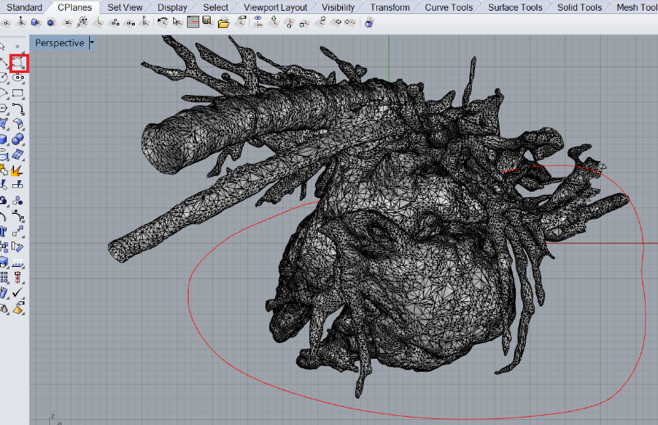
\includegraphics[width=0.75\textwidth]{Figuras/mod_03.png}
	  \caption{\emph{Modelo 3d suavizado}}
	\end{center}
	\label{fig:mod_03}
	\end{figure}

Pese a todo, a veces no nos interesa realizar la impresión 3D de todo el modelo, pero queremos contar con todo para el trabajo anterior sobre el ordenador. En este caso, realizar un proceso de segmentación es la opción más correcta. Mediante programas como \href{https://www.rhino3d.com/}{Rhinoceros} se pueden diferenciar capas dentro de un mismo modelo, y empleando la opción \emph{Mesh Split} se puede dividir el modelo en partes y asociarlo a las capas creadas anteriormente. De esta manera, podemos aplicar diferentes colores en función de la capa y ver, por ejemplo, partes oxigenadas y partes desoxigenadas del mismo modelo de forma clara.\\

	\begin{figure}[!ht]
	\begin{center}
	  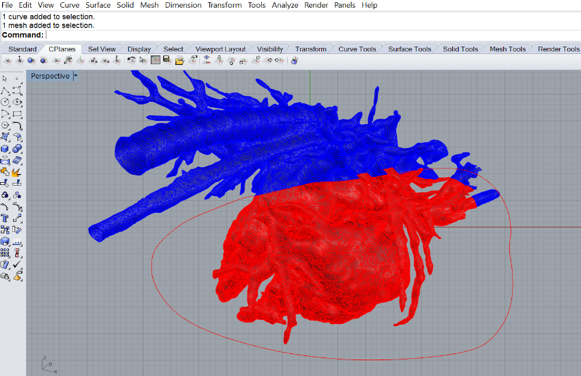
\includegraphics[width=0.75\textwidth]{Figuras/mod_04.png}
	  \caption{\emph{Modelo 3d estableciendo capas}}
	\end{center}
	\label{fig:mod_04}
	\end{figure}

	\begin{figure}[!ht]
	\begin{center}
	  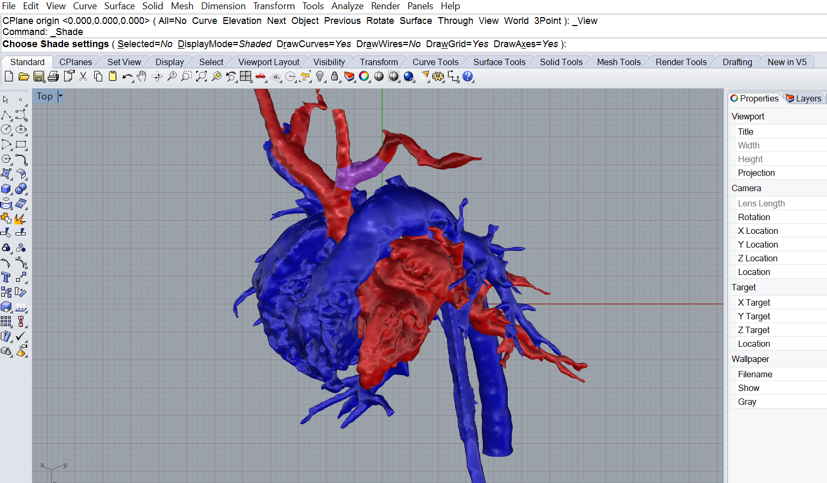
\includegraphics[width=0.75\textwidth]{Figuras/mod_05.png}
	  \caption{\emph{Modelo 3d resultado final}}
	\end{center}
	\label{fig:mod_05}
	\end{figure}

De forma esquemática, podemos resumir el proceso explicado en los puntos de la Figura \ref{modeloCardio}.\\

	\begin{figure}[!ht]
	\begin{center}
	  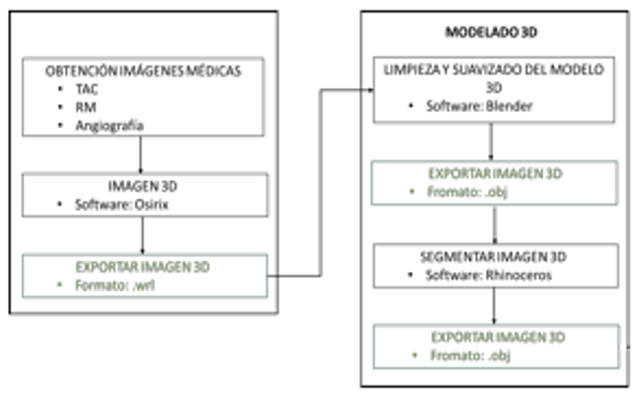
\includegraphics[width=0.5\textwidth]{Figuras/modeloCardio.png}
	  \caption{\emph{Proceso propuesto de modelado cardíaco}}
	\end{center}
	\label{modeloCardio}
	\end{figure}

\subsubsection{Modelado de Stents}
De una manera muy diferente se crean los modelos de Stents. Teniendo en cuenta las adaptaciones que deben tenerse en cuenta para imprimirlos, el proceso de diseño no seguirá un modelo que se visualice fácilmente.\\

En primer lugar deberemos considerar la cantidad de puntos que queremos que tenga el Stent así como como la longitud que tendrá. El diámetro del Stent vendrá dado por la barra donde se imprimirá, aunque este valor también debe tenerse en cuenta en el momento de crear el modelo.\\

Teniendo la impresora configurada con la barra en vez de con mesa, el eje $y$ estará destinado a la rotación de esta. No obstante, actualmente los programas empleados no estan pensados para diseñar con este ajuste, por lo que deberemos diseñar el modelo teniendo en cuenta que avanzar en el eje $y$ implica rotar la barra.\\

Finalmente, considerando las variables que tiene el diseño, nos pueden quedar modelos tales como los de la figura \ref{fig:modeloStents}.

	\begin{figure}[!ht]
	\begin{center}
	  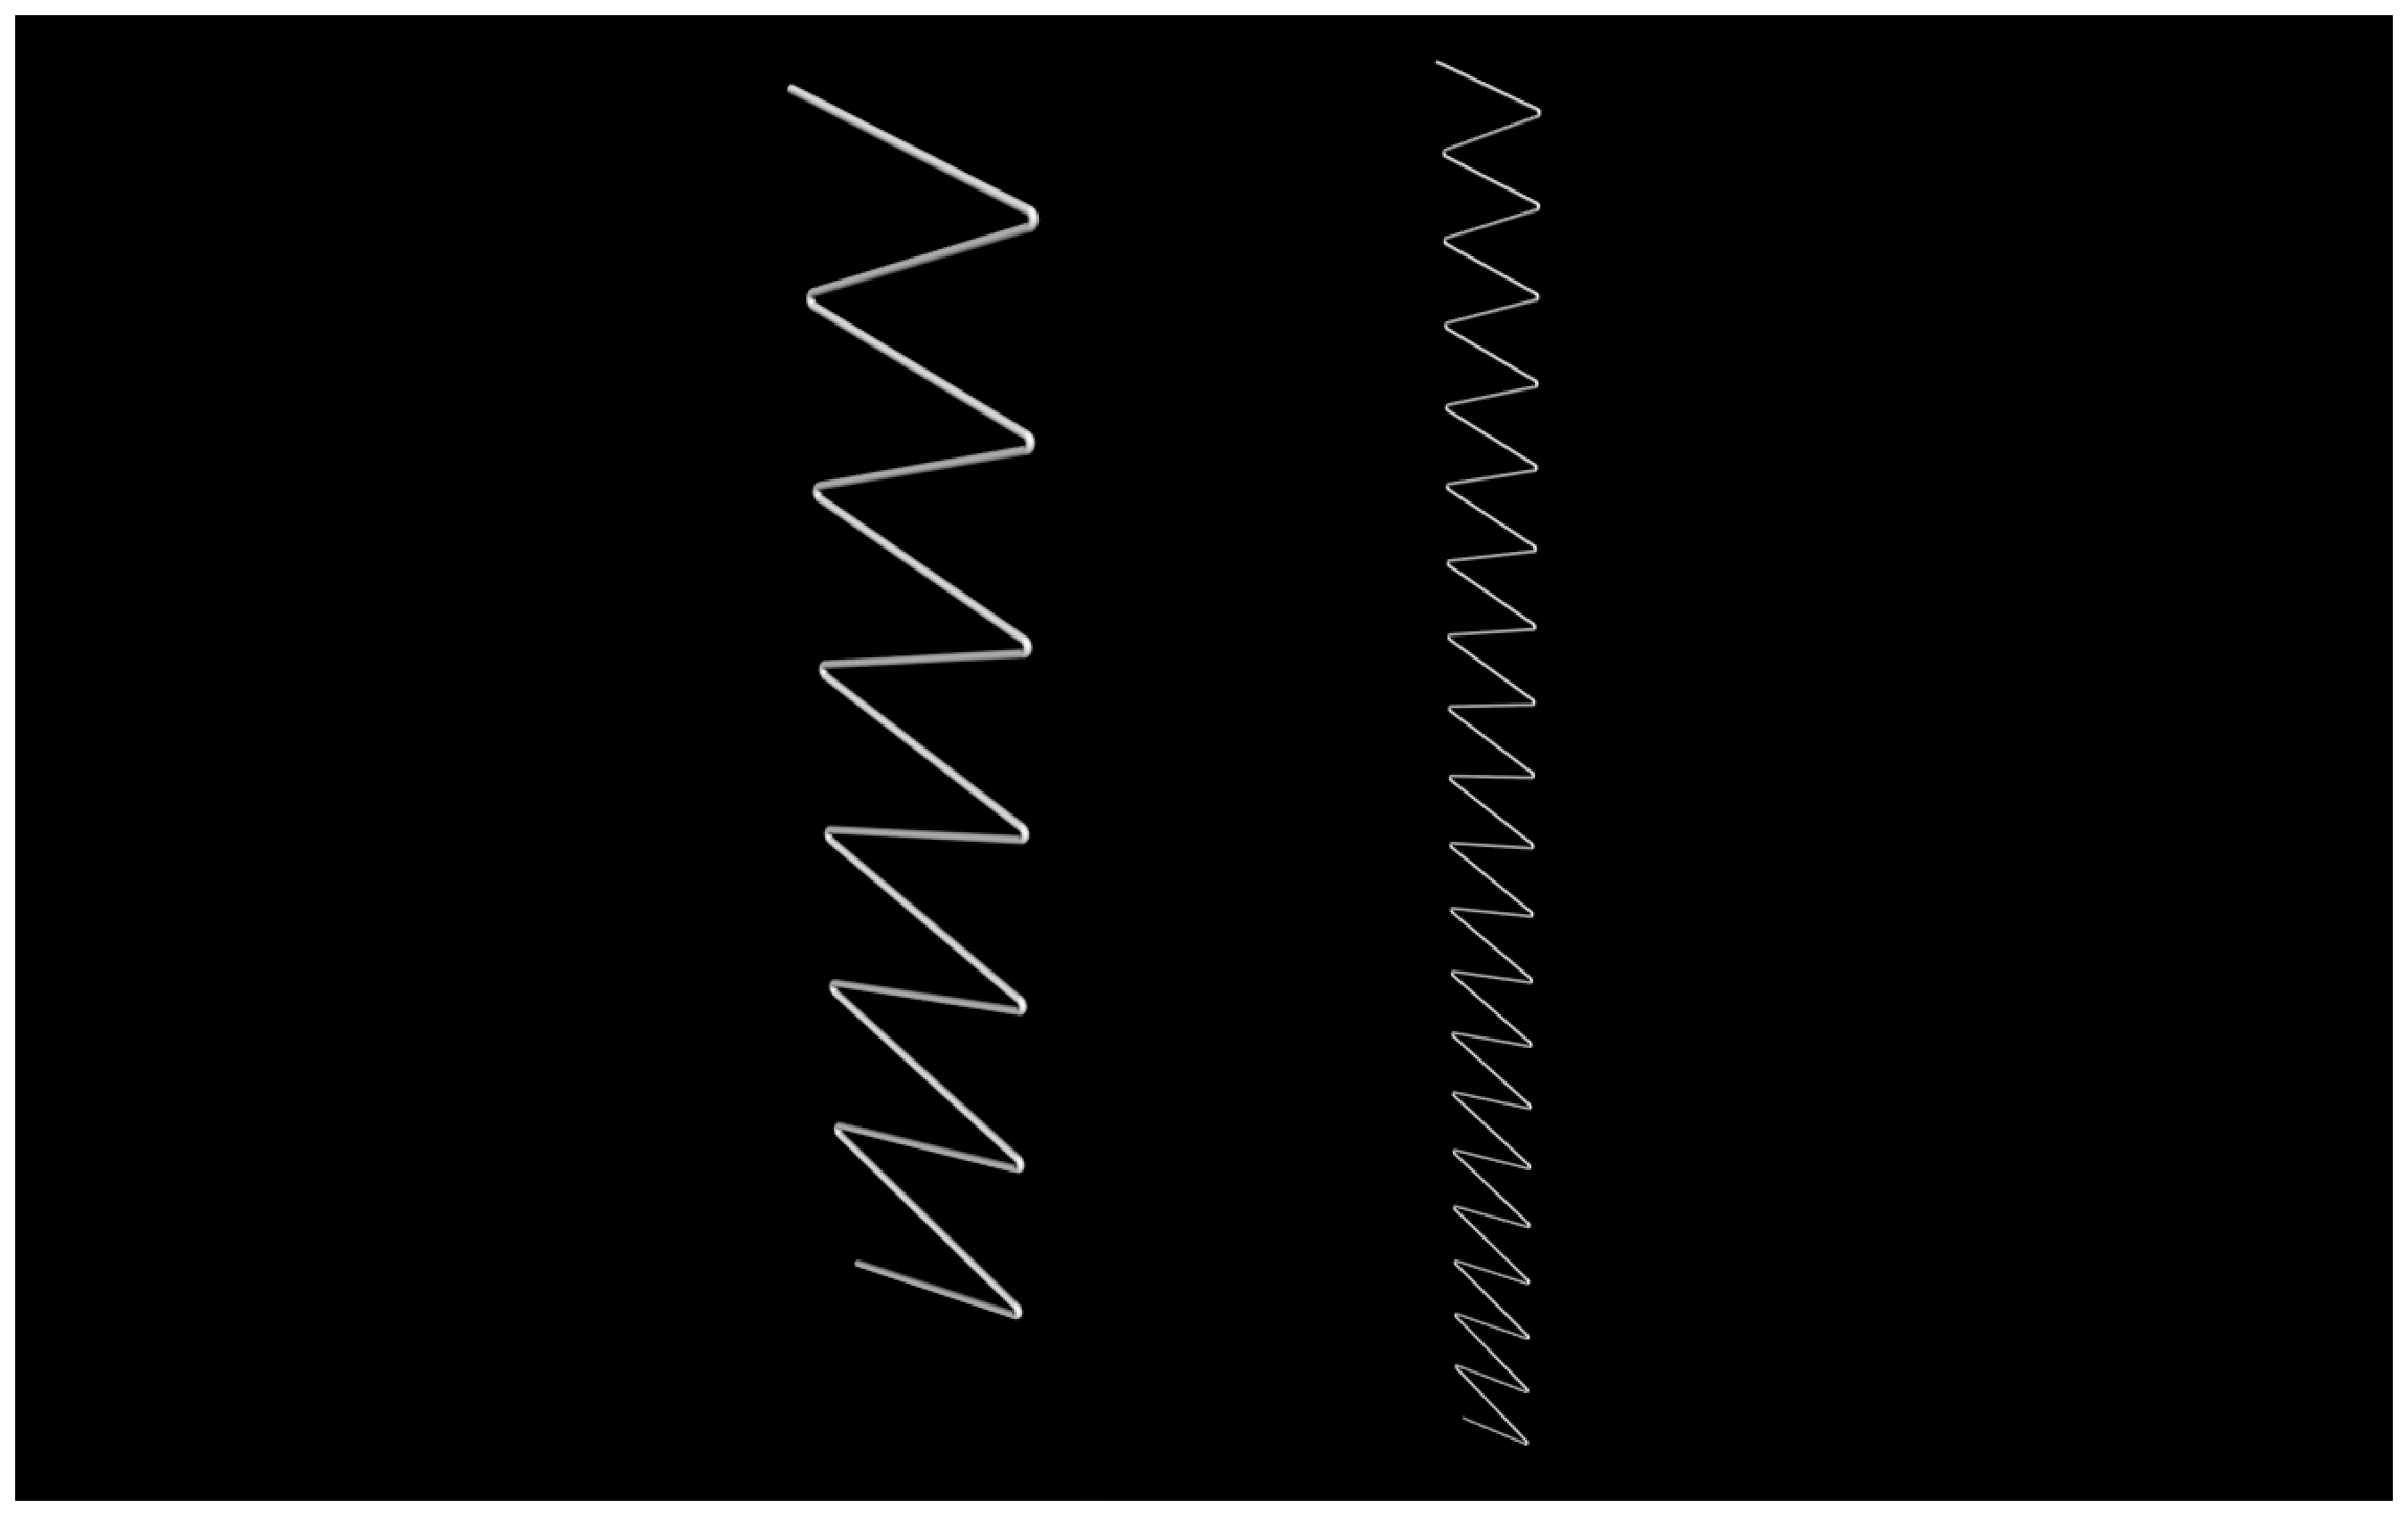
\includegraphics[width=0.75\textwidth]{Figuras/modeloStents.eps}
	  \caption{\emph{Modelos de diseño de Stents en función de los puntos}}
	\end{center}
	\label{fig:modeloStents}
	\end{figure}

Para la creación de este modelo no es necesario tener en cuenta los nudos en los que el hilo cruzará con otra línea de hilo ya creada, pues por la cantidad de material que extruye y la precisión de este el cabezal pasará por encima de la línea anterior dejando un excedente de material prácticamente insignificante.\\

\FloatBarrier
\subsection{Slicing y preimpresión}
Una vez tenemos la impresora instalada y funcional, y tenemos un modelo creado, todavía faltará hacer una serie de pasos para mandar la información a la impresora y que esta empiece a hacer su trabajo. Estos pasos consisten, básicamente, en convertir los datos del modelo a una serie de código "simplificado" con las instrucciones que debe seguir la impresora paso a paso.

Ya teniendo el modelo, el primer paso a seguir es pasarlo por un programa troceador o \emph{slicer}. Este tipo de programas reconocen los modelos y su función esencial es dividirlos en capas para que la impresora pueda ir haciéndolas una a una. Aunque varía en función del programa que se emplee, predomina en la comunidad exportar los modelos en formato \emph{.stl} para que puedan ser reconocidos por los diferentes slicers.\\

Pese a la amplia variedad de opciones disponibles, los slicers más empleados son \emph{Cura} (respaldado por el gigante Ultimaker), \emph{Slic3r} (empleado por ejemplo en el laboratorio del Dr Giuseppe Scionti), o Simplify3d (a diferencia de los anteriores, de pago).\\

Los slicer reconocen que el diseño esté bien creado, es decir, que no tenga capas sin cerrar, y detectan las partes "interiores" de los solidos. Mediante esta detección se pueden establecer diferentes parámetros, como qué grado de relleno debe tener en las partes interiores, qué patrón debe seguir (lineal, "panel de abeja", etc.) o qué grueso deben tener las paredes exteriores.\\

Asimismo, desde estos se realizarán los ajustes de impresión. Los más básicos son la temperatura a la que deben trabajar el extrusor y la cama caliente (en caso de que estén presentes en el modelo, así como podría ajustarse la temperatura de un segundo extrusor), la velocidad de movimiento que se tendrá, velocidades de los ventiladores o altura que se debe recorrer en el eje z por cada capa. Citar que cuando se trabaja con extrusión por bobina de hilo, la temperatura óptima de trabajo varía en función del material con el que estemos trabajando y por la empresa que lo haya fabricado, siendo una buena práctica acceder a la página del fabricante a buscar a qué temperatura recomiendan trabajar en caso de que no esté especificado en la bobina. Hay que tener en cuenta que, además, se pueden establecer cambios en todas las variables previamente citadas a medida que van avanzando las capas.\\

En función del programa y del tipo de conexión que tengamos establecido, podremos enviar directamente desde el slicer las órdenes de impresión a la impresora, o bien exportar estos ajustes a un archivo para que lo reciba a través de otros métodos (como la tarjeta SD). En caso de trabajar con archivo, será habitual trabajar con un archivo \emph{.gcode} que será el que el controlador Arduino interpretará. Estos archivos pueden ser abiertos y modificados desde cualquier editor de texto, y suelen incorporar ciertos comandos en la parte inicial para realizar un ajuste de la impresora, consistiendo básicamente en un proceso de calibración.\\

El estándar Gcode es creado y mantenido por la comunidad RepRap. Haciendo uso de \href{https://thingiverse-production-new.s3.amazonaws.com/assets/87/b0/2c/f5/4c/CheatSheet.pdf}{Cheat Sheets} podemos modificar el código que nos haya creado el slicer para realizar, por ejemplo, una calibración de varios puntos de la cama en vez de calibrar a un solo punto, o eliminar líneas para empezar en una posición concreta en caso de que la impresión haya fallado previamente y queramos recuperar el trabajo desde el punto en que se cortó. 



\pagebreak
\section{Implementación}


\pagebreak
\section{Práctica}
\subsection{Impresión de Stents}
Por tal de comprobar la función práctica de este trabajo, en la visita que se realizó al laboratorio del Dr Scionti se procedió a la impresión de stents cardiovasculares. Estos cuentan con todas las funcionalidades y modificaciones que se han ido citando en este proyecto anteriormente.\\

Se realizaron dos impresiones, en las cuales se crearon dos modelos de stent diferentes. Se puede visualizar el proceso de impresión de uno de ellos en el siguiente enlace: %%%% INSERTAR ENLACE!!!!!! %%%%%%%

El primer punto importante es, tras realizar la adaptación de la barra en sustitución de la cama, hacer su calibración. Hay que comprobar que la barra (en este caso, de fibra de carbono) no está torcida, y será preferible trabajar en la parte más adecuada. Teniendo ese lugar, es aconsejable realizar un ajuste del eje $z$, colocando la punta de extrusión en la posición en la que deberá trabajar en la barra y especificar ese punto como base o cero.\\

Una vez tenemos la impresora calibrada podemos proceder a la impresión de los stents.
	
	\begin{figure}[!ht]
	\begin{center}
	  \includegraphics[width=0.5\textwidth]{Figuras/stents_printing.jpg}
	  \caption{\emph{Proceso de impresión de un stent cardiovascular}}
	\end{center}
	\label{stents_printing}
	\end{figure}

Finalmente, cuando se ha acabado de imprimir, podremos proceder a sacar el stent de la barra. Al estar disuelto en cloroformo, seca de manera casi inmediata. Así pues, cuando acaba tendremos que sacar la barra de los cojinetes y extraer el stent por un extremo de esta.\\

En la figura \ref{stents_all} podemos observar diferentes tipos de stents, que varían en función del diámetro, longitud o cantidad de puntos.

	\begin{figure}[!ht]
	\begin{center}
	  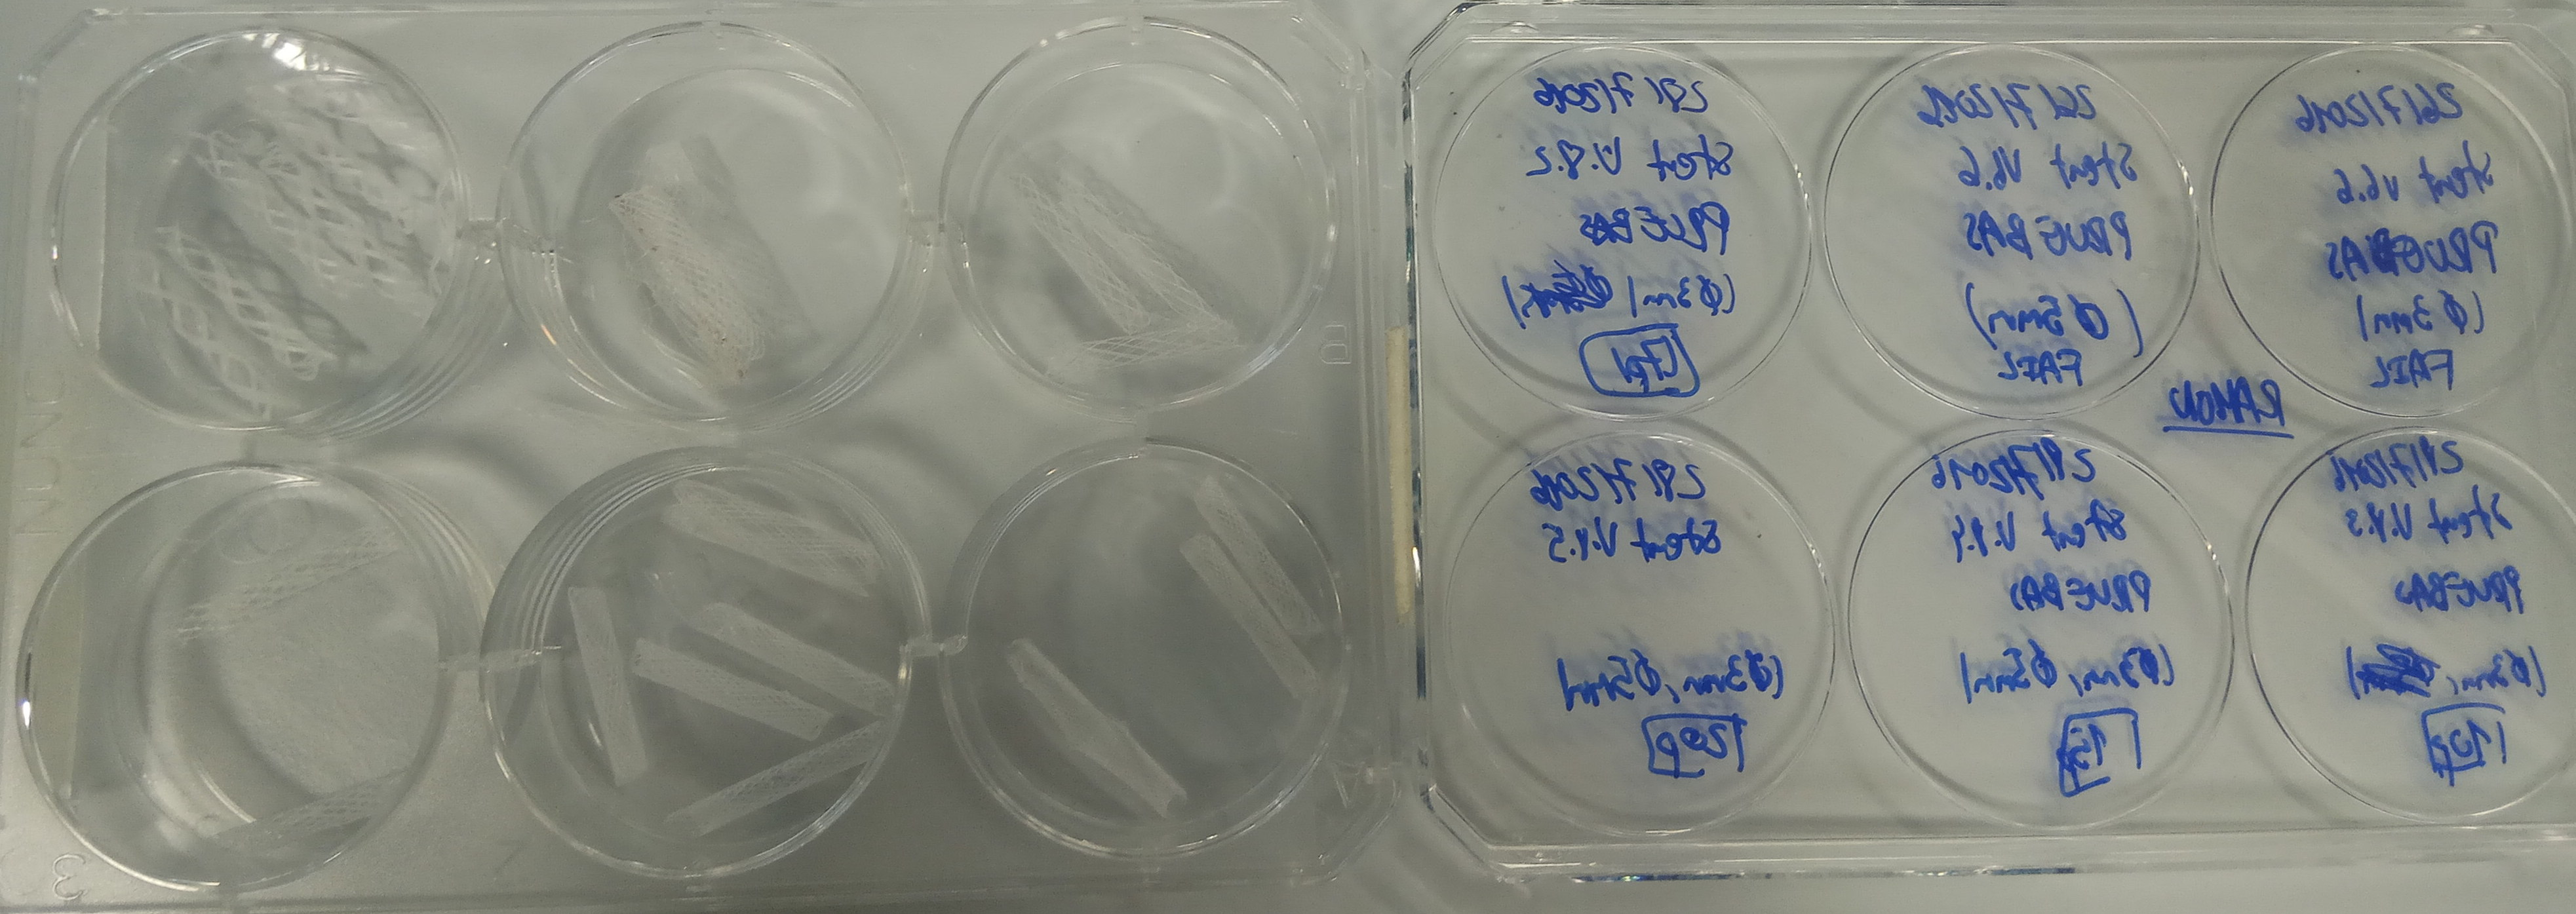
\includegraphics[width=0.5\textwidth]{Figuras/stents_all.jpg}
	  \caption{\emph{Ejemplos de stents cardiovasculares}}
	\end{center}
	\label{stents_all}
	\end{figure}

\subsection{Simulación de impresión}
Más allá del proceso de obtención de modelos virtuales en 3d está la parte de la propia impresión. Aunque no hemos podido contar con una bioimpresora para realizar pruebas, se han realizado varias pruebas con una impresora 3d convencional por tal de comprobar la importancia que tiene elegir bien las propiedades de impresión en función de cada material. Los materiales empleados para el estudio de este apartado son PLA, ABS y TPE (Thermoplastic Elastomer).\\

\paragraph{PLA}
La impresión de PLA ha sido realizada con una bobina \href{https://store.bq.com/es/bobina-pla-bq/}{PLA Premium BQ}.\\

Se ha imprimido sin base, con soportes, a temperatura de cama de 60ºC, temperatura de extrusión de 230ºC, velocidades de movimiento 70/120 mm/s, 15\% de relleno y 0.15mm de altura de capa.\\

Tras 9h de impresión, el resultado obtenido es satisfactorio. No hay signos de levantamiento de base (o \emph{warping}) y la definición, aunque pueden diferenciarse las capas, es correcta. No obstante, los soportes estan muy bien adheridos y es complicado sacarlos.\\

Para evitar el problema de los soportes, sería buena opción intentar imprimir la pieza con menor temperatura de extrusión y con velocidades de movimiento menores. También podría ser recomendable imprimir con un porcentaje de relleno mayor.

	\begin{figure}[!ht]
	\begin{center}
	  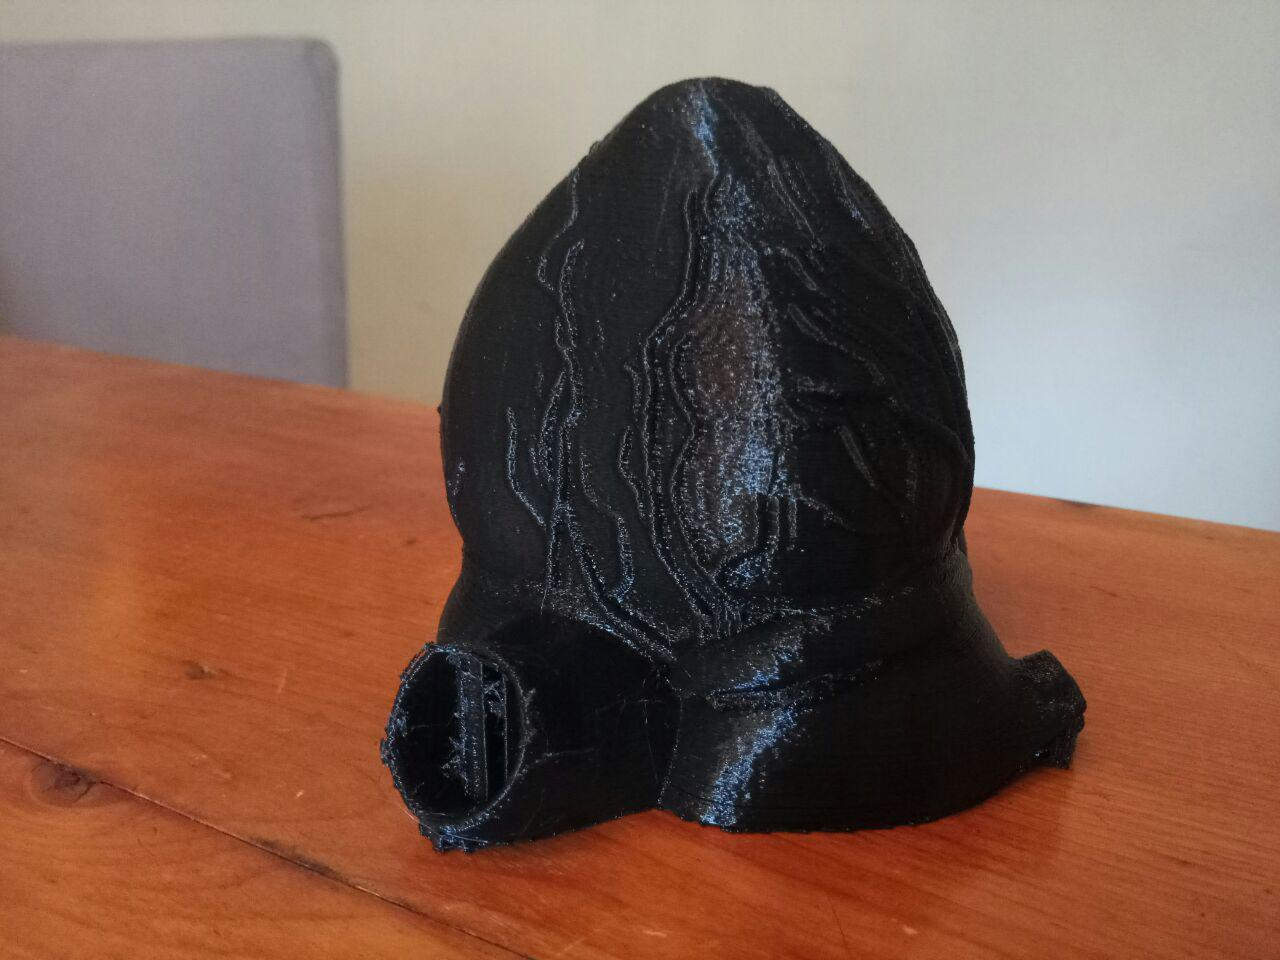
\includegraphics[width=0.5\textwidth]{Figuras/heart3.jpg}
	  \caption{\emph{Impresi\'{o}n en PLA}}
	\end{center}
	\label{heartPLA}
	\end{figure}


\paragraph{TPE}
La impresión de TPE ha sido realizada con una bobina \href{http://www.nunus-filamente.com/filamente/product/nunus-flexible-rubber-filament-175mm-1kg-rot/}{NuNus Flexible Rubber Filament}.

A diferencia de con PLA, la temperatura de la cama es menor, y la velocidad de extrusión debe ser rebajada considerablemente. Respecto a los parámetros del PLA, ha sido imprimido con una temperatura de extrusión de 230ºC y 30ºC de cama mientras que la velocidad de impresión es de 30mm/s y 70mm/s para transporte. Otro cambio considerable es que se ha creado con estructuras de base, con \emph{raft}.\\

En este caso podemos observar claramente que ha aparecido warping, pues al poner la figura en plano presenta curvatura. Se puede ver también que hay capas que no se han acabado de fundir y, por tanto, no presentan correcta adhesión entre las líneas. Asimismo, al haber aparecido warping, el extrusor se ha encontrado con material en puntos donde debería imprimir; debido a este suceso, cuando en estos puntos se imprimían estructuras de soporte, estas se han adherido con mucha fuerza al modelo, resultando muy complicado extraerlas posteriormente.\\

Se puede apreciar que la dificultad que presenta imprimir con TPE respecto al PLA es mucho mayor, invirtiendo un tiempo mucho mayor para la impresión y unos resultados menos definidos.

	\begin{figure}[!ht]
	\begin{center}
	  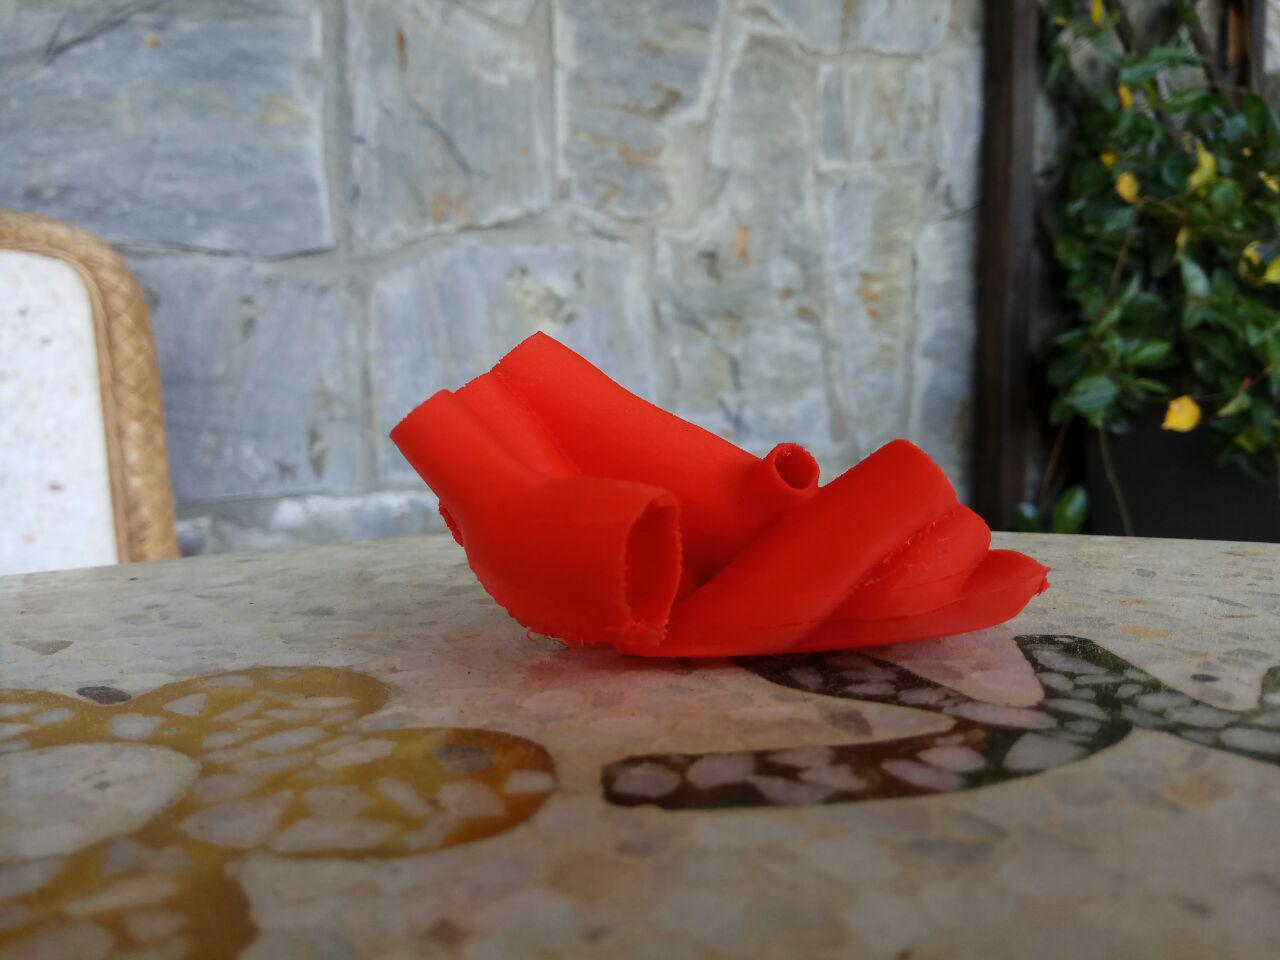
\includegraphics[width=0.5\textwidth]{Figuras/heart1-1.jpg}
	  \caption{\emph{Impresi\'{o}n en TPE: warping}}
	\end{center}
	\label{heartTPE1}
	\end{figure}

	\begin{figure}[!ht]
	\begin{center}
	  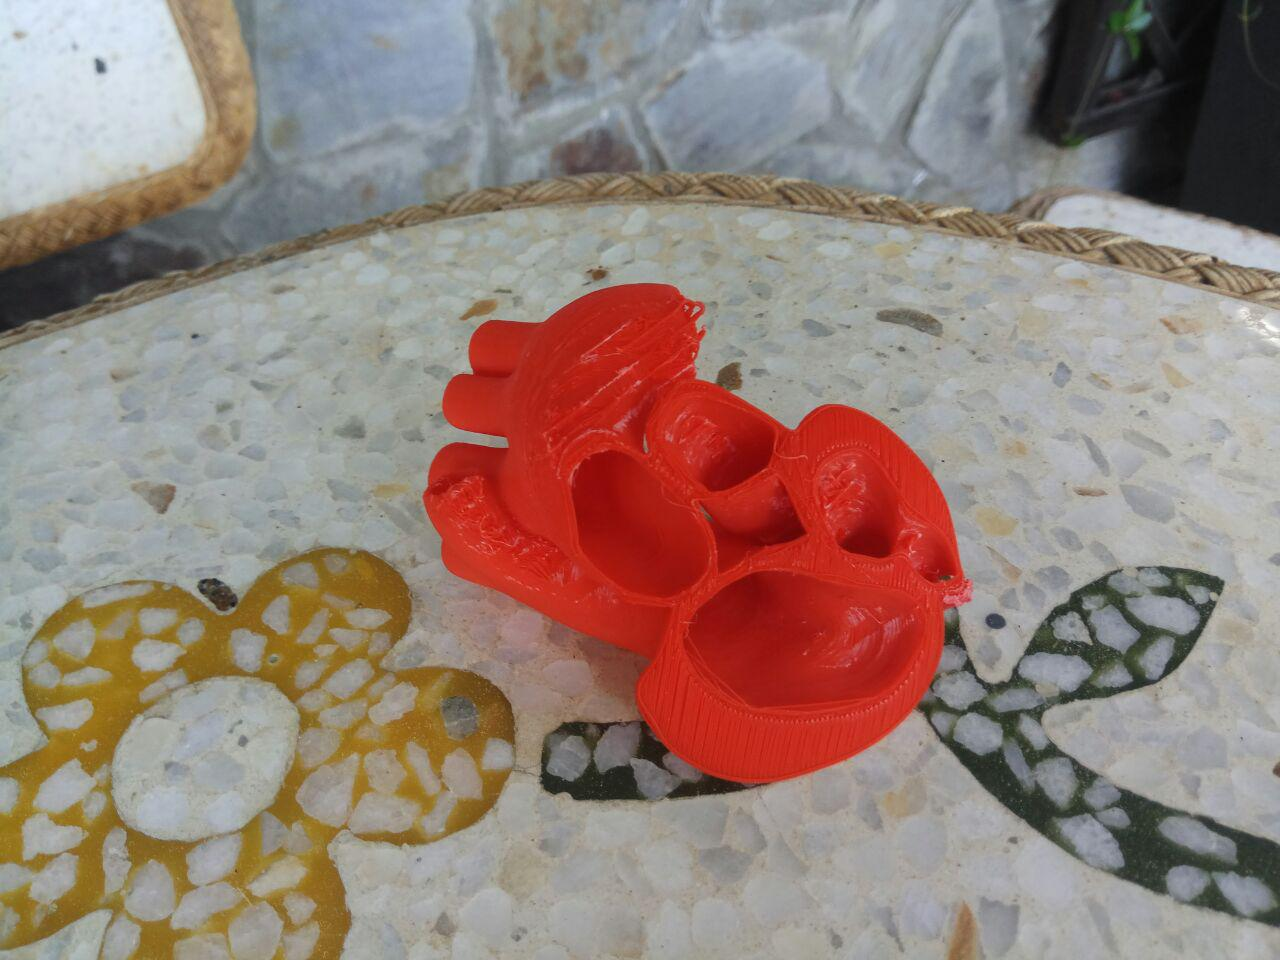
\includegraphics[width=0.5\textwidth]{Figuras/heart1-2.jpg}
	  \caption{\emph{Impresi\'{o}n en TPE: soportes}}
	\end{center}
	\label{heartTPE2}
	\end{figure}


\paragraph{ABS}



\subsection{Propuestas de mejora}



\pagebreak
\section{Proyección}

\pagebreak
\section{Conclusiones}


\pagebreak
\section{Bibliografía}


\pagebreak
\section{Anexos}

\end{document}
